\section{Rete prodotti}\label{ReteProdotti}
L'analisi condotta sulla rete ha lo scopo di individuare gruppi di prodotti che interagiscono tra loro e di andare ad individuare quelli più strategici all'interno della rete tramite un'analisi di centralità. Nel seguito vengono descritte le scelte di costruzione della rete, definito il concetto di prodotto strategico ed infine presentate le analisi che partendo dalla globalità della rete scendono nei dettagli delle sottoreti più significative. 

\subsection{Costruzione rete}
Inizialmente sono state generate 3 reti diverse tenendo conto delle singole relazioni \textit{bought\_together}, \textit{also\_bought} e \textit{also\_viewed}. Da un studio generale è emerso che la relazione \textit{also\_viewed} risulti poco significativa per gli obiettivi preposti, per cui è stata scartata in quanto collega prodotti prettamente simili tra loro. Le relazioni di\textit{bought\_together} e \textit{also\_bought}, invece, permettono di portare alla luce prodotti diversi il cui impiego effettivo può dipendere l'uno dall'altro e ciò permette di stabilire se esistono prodotti particolarmente strategici all'interno della rete. Si è inoltre notato che le due relazioni in questione riportano spesso lo stesso prodotto come sia in \textit{bought\_together} che in \textit{also\_bought} e che inoltre la direzionalità della relazione \textit{also\_bought} sia indipendente da una temporalità di acquisto. \\
Al netto di queste motivazioni, è state considerato ragionevole effettuare un'unione delle due relazioni in un'unica relazione di acquisto adirezionale. 
\\\\
Una volta stabilito il nuovo insieme di relazioni è stata necessaria una fase di pulizia per andare a scartare gli archi e i nodi superflui per la costruzione della rete. Per prima cosa è stato necessario rimuovere tutti gli archi di cui non sono presenti le informazioni relative al nodo destinazione. Dopodichè, sono state unite tutte le relazioni simmetriche in quanto la direzionalità delle relazioni non è significativa ai fini di questa analisi. Infine, sono stati rimossi dalla tabella dei prodotti tutti i nodi rimasti isolati dopo il filtraggio delle relazioni. Al termine del processo di pulizia si è passati da 82628 a 26572 per il numero di archi e da 20459 a 17914 per il numero di nodi. \\
A partire dal nuovo insieme di archi è stata quindi costruita la rete dei prodotti tramite un grafo non orientato.



\subsection{Concetti di prodotto centrale}
In questa analisi con il termine \textbf{prodotto strategico} si intende quel prodotto che, se pubblicizzato in base a quanto emerge dalla rete, può costituire delle vendite facili verso chi acquista altri prodotti correlati ad esso. \\
I prodotti strategici vengono individuati tramite il calcolo delle centralità dei nodi. In particolare, è la \textit{degree centrality} quella che permette di individuare i prodotti che hanno maggiori interazione con altri. Trovare un prodotto con centralità di grado alta significa trovare un prodotto con un ampio vicinato. Per questo motivo se si dovesse scegliere quali prodotti pubblicizzare a partire da uno specifico nodo, una scelta strategica potrebbe essere quella di dare priorità ai prodotti del vicinato con grado più alto. Questa misura di centralità sarà particolarmente per stabilire i prodotti più importanti all'interno delle sottoreti relative a categorie e communities. \\\\
Una misura di centralità che può essere utile per un'analisi sulla rete nella sua globalità è quella della \textit{closeness centrality}. Tramite essa è possibile individuare i prodotti meglio posizionati per influenzare la rete più velocemente. Per esempio aggiungendo un annuncio pubblicitario sulla pagina del prodotto, esso sarà più velocemente raggiungibile dagli altri prodotti della rete seguendo una catena di acquisti.
   

\subsection{Analisi generale}
La rete che è stata costruita conta un totale di 962 componenti connesse, tra cui una giant component (figura \ref{fig:giantComponent}) costituita da 11,937 nodi e 18,991 archi. \\
In figura \ref{fig:distribuzioneGradi} è mostrata la distribuzione dei gradi. Computando l'average degree (2.966) si osserva che mediamente un prodotto tende ad essere connesso con altri 3 prodotti. Il coefficiente di clustering medio dell'intera rete è pari a 0.286, quindi mediamente per un nodo si ha che circa 1/3 dei vicini è connesso. La densità della rete ha un valore molto basso pari, pari a 0.000165 . \\\\

\begin{figure}[]
    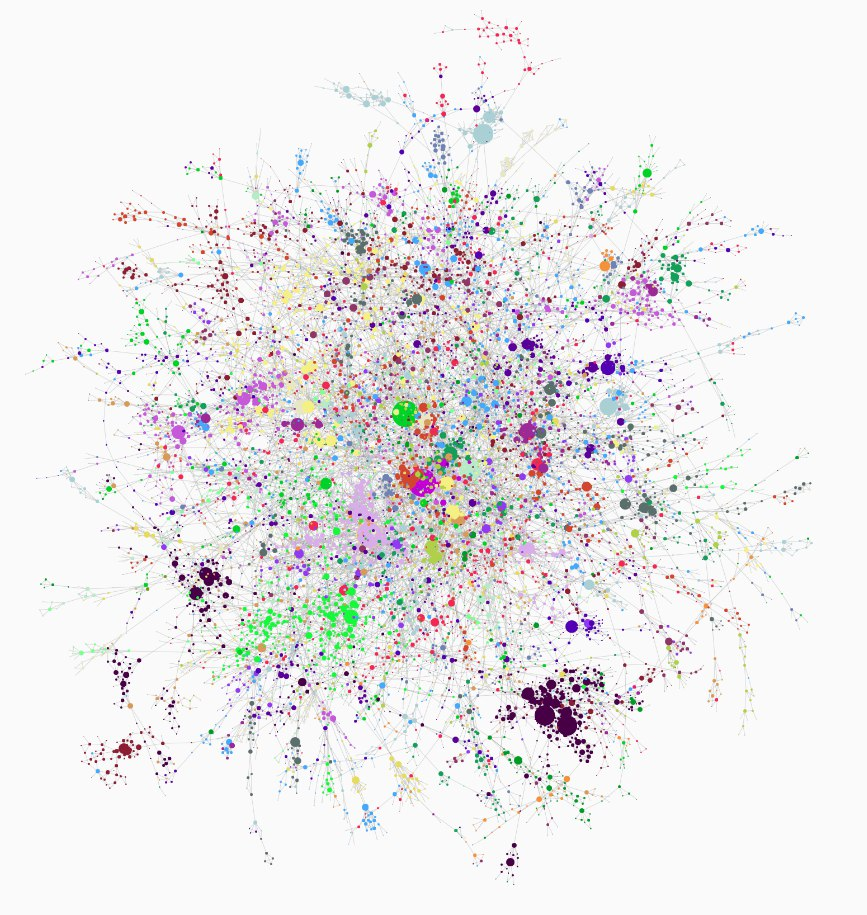
\includegraphics[scale=0.45]{giantComponent}\centering
    \caption{Giant component colorata per categorie e con dimensione dei nodi data dalla degree centrality}\label{fig:giantComponent}
\end{figure}

\begin{figure}[H]
    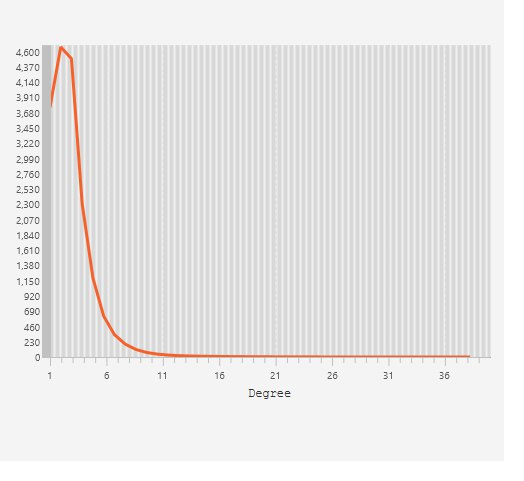
\includegraphics[scale=0.37]{distribuzioneGradi}\centering
    \caption{Distribuzione dei gradi nella rete completa}\label{fig:distribuzioneGradi}
\end{figure}

Calcolando il coefficiente di assortatività sull'intera rete si ottiene un valore di -0.0194 che, essendo negativo, permette di asserire che la rete sia di tipo disassortativo. È infatti possibile osservare nel grafico in figura \ref{fig:assortativity} come i nodi  con grado più alto, seppur in modo non nettamente marcato, tendano a connettersi a nodi con grado basso. A conferma di ciò, in figura \ref{fig:hubs} si può osservare come i nodi di grado più alto\footnote{sono stati considerati come nodi gli hubs di grado almeno pari a 20} non tendano a connettersi tra loro. È possibile quindi supporre che nella rete sono più frequenti gli acquisti di prodotti con centralità di grado alta e in combinazione con prodotti di bassa centralità. Data la natura della rete, la rimozione di un prodotto hub potrebbe quindi portare ad isolare i prodotti con grado basso. 

\begin{figure}[H]
    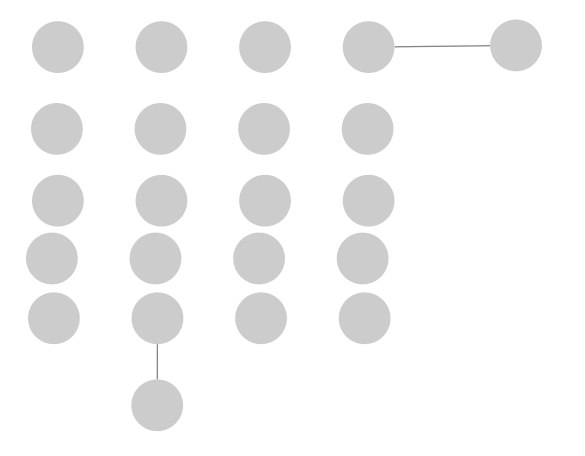
\includegraphics[scale=0.3]{hubs}\centering
    \caption{Nodi hubs con grado almeno pari a 20 isolati dal resto della rete}\label{fig:hubs}
\end{figure}

\begin{figure}[H]
    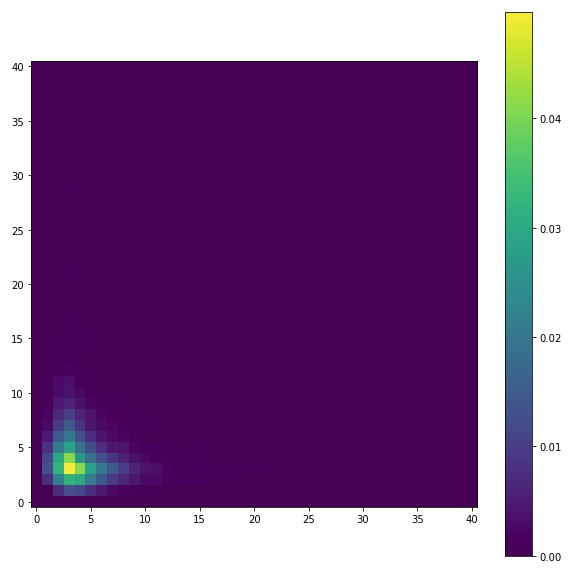
\includegraphics[scale=0.37]{assortativity}\centering
    \caption{Grafico di degree correlation}\label{fig:assortativity}
\end{figure}

In tabella \ref{tab:topDegreeFullNetwork} sono riportati i prodotti centrali della rete in termini di grado, ossia quelli definiti precedentemente come prodotti strategici. \\
In tabella \ref{tab:topClosenessFullNetwork} sono invece riportati i prodotti centrali della rete in termini di closeness. \\

%TODO: tab:topDegreeFullNetwork
%TODO: tab:topClosenessFullNetwork


\subsection{Analisi categorie}
Dopo aver osservato la rete nella sua globalità si è deciso di osservare le interazioni tra i prodotti dividendo la rete rispetto alle categorie. I risultati mostrati sono quelli relativi alle categorie più grandi in quanto, avendo a disposizione una porzione non bilanciata del dataset dei prodotti di amazon, sono le più significative. 
\\\\
In tabella \ref{tab:categoriesStats} sono disponibili le statistiche estratte per le prime 5 categorie più popolate. Per ogni categoria viene indicato il totale dei prodotti da cui è composta e il prodotto più centrale rispetto alla degree centrality con il rispettivo grado. \\
Prendendo per esempio il nodo centrale della categoria \textit{kitchen}, esso corrisponde al prodotto di un asse da stiro. Verificando i prodotti del suo vicinato, ossia quelli comprati spesso in combinazione con lo stesso, si osserva che sono per lo più ferri da stiro. Questo è un chiaro esempio di come il prodotto centrale in termini di grado sia in realtà un prodotto accessorio rispetto al suo vicinato. Essendo quindi un prodotto comune per diversi prodotti principali può essere considerato un prodotto strategico data la sua più facile vendibilità. \\
Un comportamento analogo è stato riscontrato anche per molti altri prodotti con degree centrality maggiore.
\\\\
Osservando come si dispongono nella rete le diverse categorie, si può notare che una stessa categoria vada a formare gruppi distinguibili di prodotti. In figura \ref{fig:musicalInstruments} è riportato l'esempio per la categoria \textit{musical-instruments}. Per questo motivo, come si vedrà nella sezione successiva, è stata effettuata in seguito un processo di community detection sulla rete per individuare i reali gruppi di prodotti che si formano in base alle relazioni di acquisto.

\begin{figure}[]
    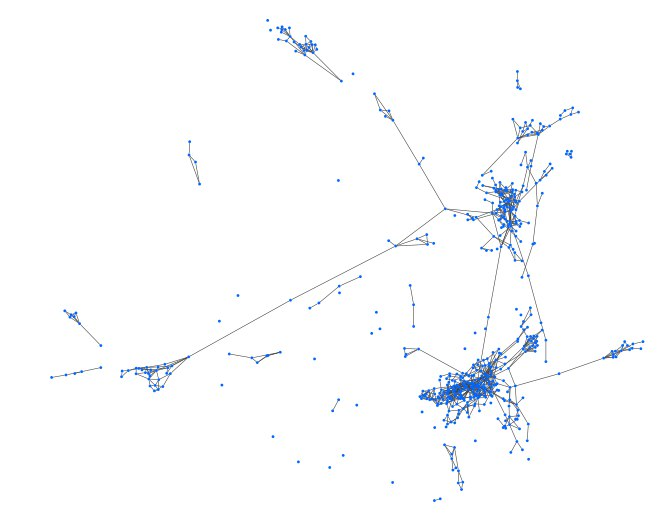
\includegraphics[scale=0.35]{musicalInstruments}\centering
    \caption{Sottorete dei prodotti della categoria musical-instruments}\label{fig:musicalInstruments}
\end{figure}

\subsection{Analisi communities}
Le communities della rete sono state individuate mediante l'algoritmo Clauset-Newman-Moore greedy modularity maximization. Tramite questo algoritmo sono state trovate 1064 communities. Il numero elevato era prevedibile data la grande quantità pari a 962 delle componenti connesse. Si è osservato, inoltre, che le communities più rilevanti fanno tutte parte della giant component, la quale ne contiene 103. \\\\
Come per le categorie, i risultati mostrati sono quelli relativi alle communities più importanti. 
\\\\
In tabella \ref{tab:communitiesStats} sono disponibili le statistche estratte per le prime 10 communities. \\
Oltre a fornire la cardinalità e gli elementi centrali come per le categorie, per ogni community è stato calcolato il coefficiente di clustering medio per determinare il livello di coesione.  Inoltre ci si è posti l'obiettivo di identificare la sfera di interesse di ogni gruppo di prodotti e di darne una sorta di etichetta che possa riassumerne il contenuto. A tale scopo sono stati calcolati i seguenti campi:
\begin{itemize}
    \item \textbf{dominant category}: categoria dominante della community; calcolata come %TODO: zscore by rpo il bibliografo
    \item \textbf{categories distribution}: distribuzione delle categorie principali presenti nella community
    \item \textbf{top words}: parole più frequenti presenti nei titoli dei prodotti di una community; %TODO: RPO dire qualcosa sul come?
    \item \textbf{top entities}: entità più frequenti estratte tramite entity recognition dai titoli dei prodotti di una community; %TODO: RPO dire qualcosa sul come?
\end{itemize}

%TODO tab:communitiesStats tabella con le top 10 communities

Nelle figure \ref{fig:wordCloud5} e \ref{fig:wordCloud7} si possono vedere rispettivamente le word clouds delle communities 5 e 7. Dalle immagini è facilmente intuibile che la prima verte su prodotti smart per la casa, mentre la seconda comprende prodotti accessori e prodotti legati alla chitarra. Ciò è confermato anche dalle entità più frequenti.

\begin{figure}[]
    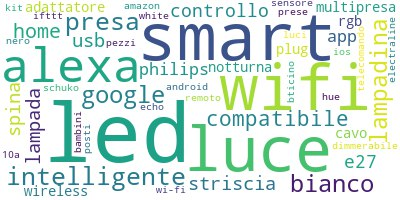
\includegraphics[scale=0.4]{wordCloud5}\centering
    \caption{Word cloud della community 5}\label{fig:wordCloud5}
\end{figure}
\begin{figure}[]
    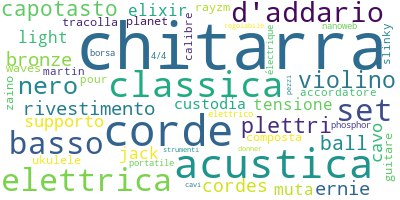
\includegraphics[scale=0.4]{wordCloud7}\centering
    \caption{Word cloud della community 7}\label{fig:wordCloud7}
\end{figure}